\documentclass{article}
\usepackage{graphicx}
\input{setup}
\usepackage{polski}
\usepackage[margin=2cm]{geometry}
\title{Złącze metal(ferromagnetyk)/nadprzewodnik. 
Odbicia Andreeva}
\author{Marta Wleklińska}
\date{\today}

\begin{document}

\maketitle

%%%%%%%%%%%%%%%%%%%%%%%%%%%%%%%%%%%%%%%%%%%%%%
\section{Wstęp}
%%%%%%%%%%%%%%%%%%%%%%%%%%%%%%%%%%%%%%%%%%%%%%
Celem ćwiczenia było zbadanie układu: metal (NM: \textit{normal metal})/nadprzewodnik (SC: \textit{superconductor}) oraz NM/SC/NM.
Ponownie korzystając z pakietu \texttt{kwant}, mogliśmy po definicji układu w przystępny sposób zbadać relację dyspersji, konduktancję, różne współczynniki odbić, etc.
%%%%%%%%%%%%%%%%%%%%%%%%%%%%%%%%%%%%%%%%%%%%%%
%%%%%%%%%%%%%%%%%%%%%%%%%%%%%%%%%%%%%%%%%%%%%%
\section{Wyniki}
%%%%%%%%%%%%%%%%%%%%%%%%%%%%%%%%%%%%%%%%%%%%%%
\subsection{NM/SC}
Ćwiczenie rozpoczęliśmy od układu NM/SC.
Dyskretyzacja równania
\begin{equation}
    \begin{bmatrix}
        -\frac{\hbar^2}{2m}{\nabla^2}+V(x)-\mu-h(x) & \Delta(x)\\
        \Delta (x) & -\left[-\frac{\hbar^2}{2m}\nabla^2+V(x)-\mu+h(x)\right]
    \end{bmatrix}
        \begin{bmatrix}
            \psi_{e}^{\uparrow}(x)\\
            \psi^{\downarrow}_{h}(x)
        \end{bmatrix}
        =
        E
        \begin{bmatrix}
            \psi^{\uparrow}_e(x)\\
            \psi_{h}^{\downarrow}(x)
        \end{bmatrix}
\end{equation}
prowadzi do wyrażenia na \texttt{onsite} oraz \texttt{hopping} kolejno
\begin{gather}
    \begin{bmatrix}
        2t + V(x) - h(x) - \mu & \Delta(x)\\
        \Delta(x) & -2t - V(x) - h(x)+\mu
    \end{bmatrix},\\
    \begin{bmatrix}
        -t & 0 \\
        0 & t
    \end{bmatrix},
\end{gather}
gdzie \texttt{t=hbar ** 2/(2m * dx ** 2)}.
Funkcje $h(x)$ oraz $\Delta(x)$ przyjmowały różne wartości w zależności od tego, czy $x$ było w obszarze NM czy SC, tj.
\begin{gather}
    h(x) = \begin{cases}
        P\mu, \quad \text{dla obszaru NM},\\
        0.0, \quad \text{dla obszaru SC},
    \end{cases}\\
    \Delta(x) = \begin{cases}
        0.0 \quad \text{dla obszaru NM},\\
        \Delta \quad \text{dla obszaru SC.}
    \end{cases}
\end{gather}
Dodatkowo, wprowadzony został potencjał rozpraszania $V(x)$ zlokalizowany na styku NM/SC w postaci
\begin{gather}
    V(x) = Z\mu \exp\left[-\frac{(x-x_{\text{center}})^2}{2a^2}\right],
\end{gather}
przy czym $x_{\text{center}}$ określa położenia styku FM/SC.\\
\\
W pierwszej części ćwiczenia, przyjęliśmy wartości $P=0.0, Z=0.0$.
Na rysunku~\ref{fig:ex1-transmission} przedstawione zostały wyniki transmisji, współczynnika odbicia~$E_{ee}$ oraz Andreeva $R_{he}$.\\
\begin{figure}[htp!]
    \centering
    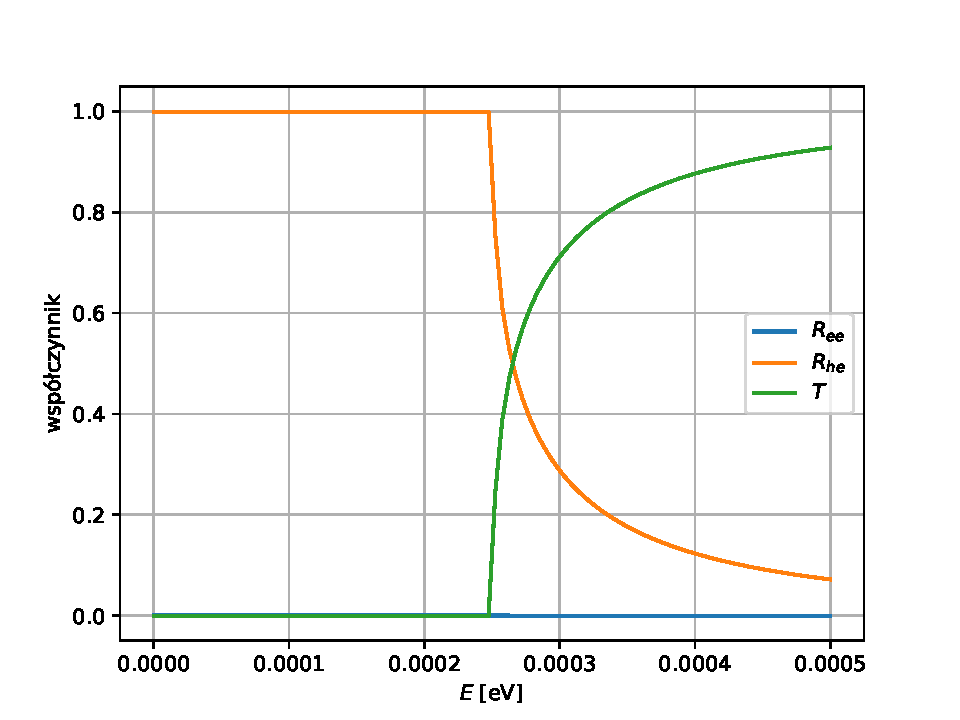
\includegraphics[width=0.65\linewidth]{ex1/ex1_transmission.pdf}
    \caption{Współczynniki transmisji w funkcji energii padającego elektronu dla złącza NM/SC.}
    \label{fig:ex1-transmission}
\end{figure}
\\
Następnie za pomocą zależności
\begin{equation}
    G(E) = \frac{e^2}{h}\left(1 - R_{ee}(E) + R_{he}(E)\right)
\end{equation}
można było wyznaczyć wyznaczyć zależność konduktancji w funkcji energii, co zostało przedstawione na rysunku~\ref{fig:ex1-conductance}
\begin{figure}[htp!]
    \centering
    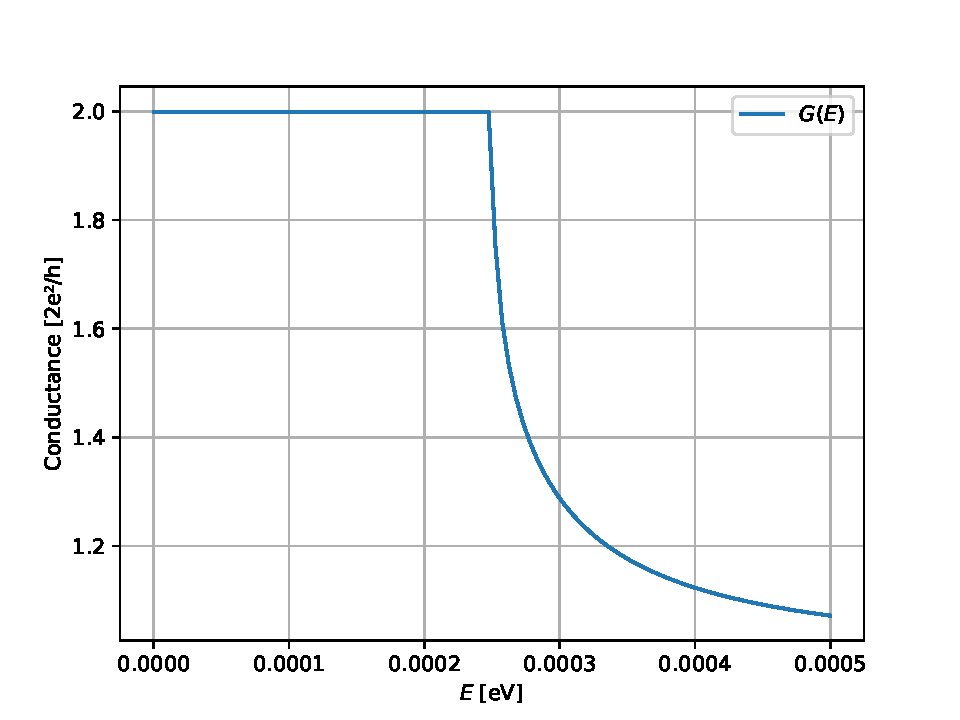
\includegraphics[width=0.65\linewidth]{ex1/ex2_conductance.pdf}
    \caption{Konduktancja w funkcji energii padającego elektronu dla złącza NM/SC}
    \label{fig:ex1-conductance}
\end{figure}
Możemy zauważyć, że podwojenie konduktancji następuje dla pewnych niższych wartości energii - później maleje ona do jedności.\\
\\
W kolejnych częściach badaliśmy wpływy parametrów $Z, P$, które mówiły o pewnych niedoskonałościach układu.
Przy niezerowym $Z$ (amplituda potencjału rozpraszania) zbadaliśmy ponownie konduktancję.
Wyniki dla wybranych $Z$ zostały przedstawione na rysunku~\ref{fig:ex1-conductance_z}.
\begin{figure}[htp!]
    \centering
    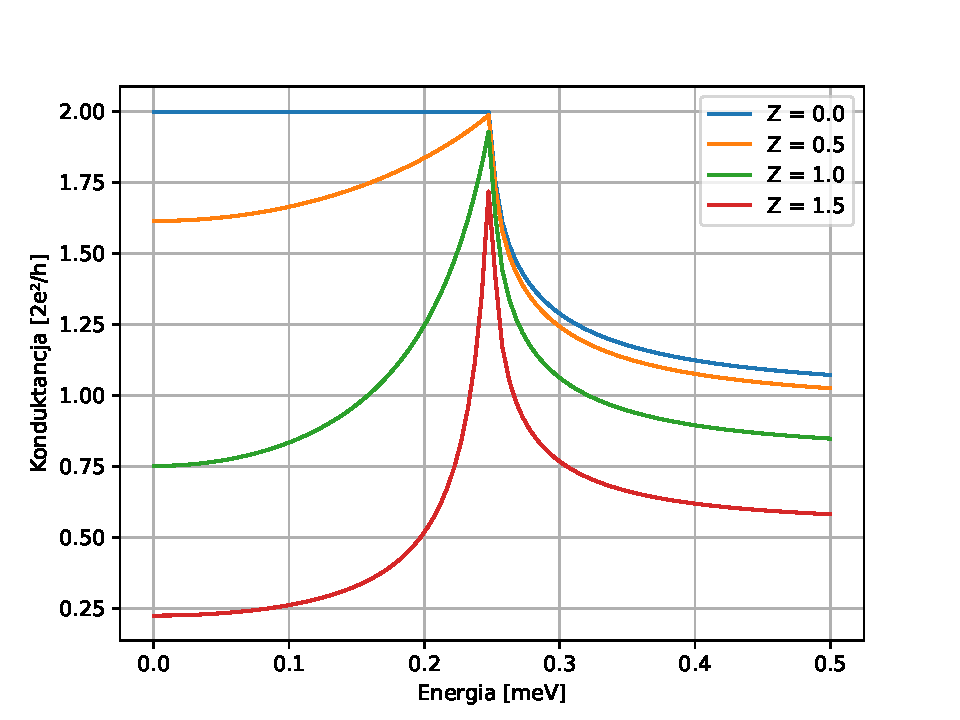
\includegraphics[width=0.65\linewidth]{ex1/ex4_conductance_vs_Z.pdf}
    \caption{Konduktancja w funkcji energii padającego elektronu dla złącza NM/SC przy założeniu różnej siły
rozpraszania na złączu.}
    \label{fig:ex1-conductance_z}
\end{figure}
Ponownie obserwujemy podwojenie konduktancji (lub prawie podwojenie) dla wszystkich rozpatrywanych przypadków, jednak występuje ono dla konkretnej wartości energii $\sim 25$~meV, co jest również szerokością przerwy nadprzewodzącej.\\
\\
Następnie przy zerowej wartości $Z$, przyjęliśmy niezerowe $P$ i wyznaczyliśmy kolejne zależności konduktancji w funkcji energii, co zostało przedstawione na rysunku~\ref{fig:ex1-conductance-P}.
\begin{figure}[htp!]
    \centering
    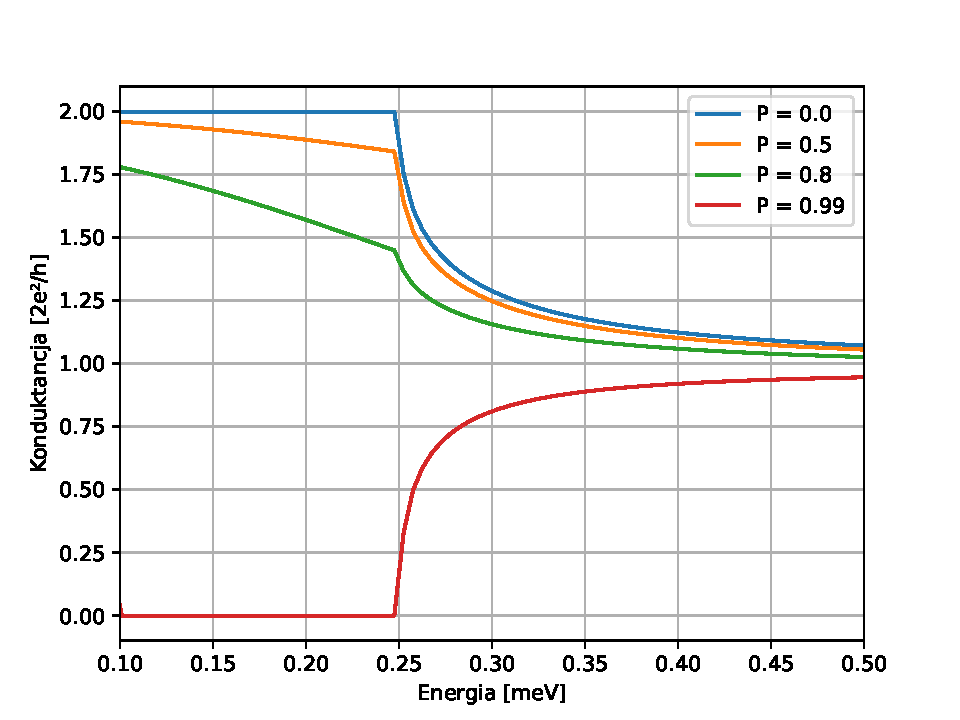
\includegraphics[width=0.65\linewidth]{ex1/ex5_conductance_vs_P.pdf}
    \caption{ Konduktancja w funkcji energii padającego elektronu dla złącza FM/SC przy założeniu różnej
spinowej polaryzacji ferromagnetyka, P}
    \label{fig:ex1-conductance-P}
\end{figure}
Obserwujemy różnice względem przypadku idealnego $P=0, Z=0$, nie obserwując kompletnego podwojenia konduktancji.\\
\\
Jako ostatnią zależność, zbadaliśmy ponownie współczynniki odbicia, transmisji w funkcji $P$, co zostało zapisane na rysunku~\ref{fig:ex1-conductance-e-06}.
\begin{figure}[htp!]
    \centering
    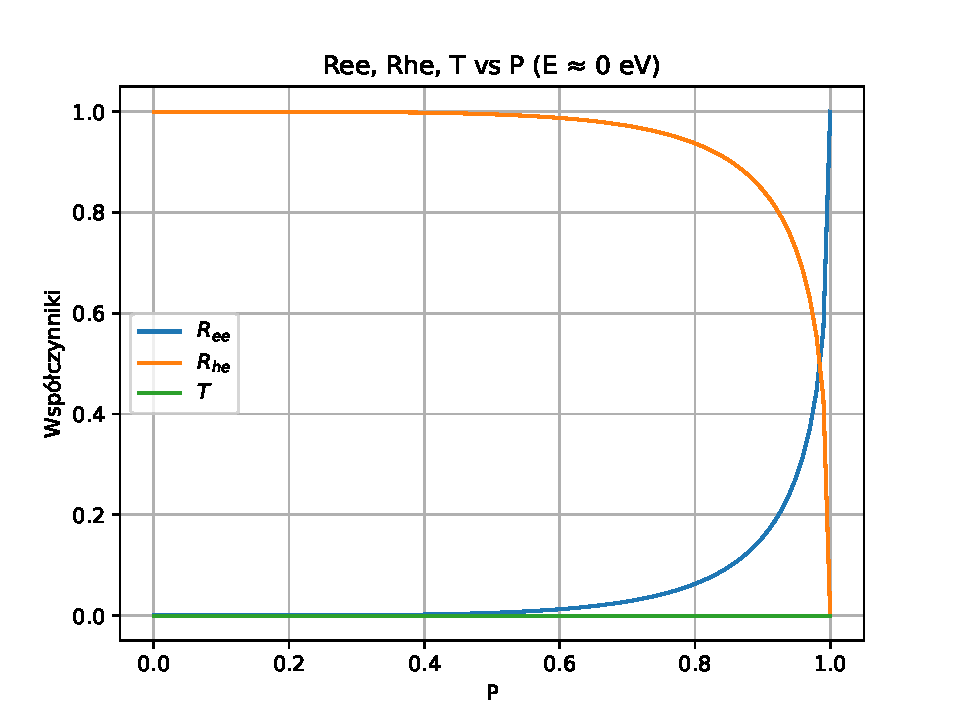
\includegraphics[width=0.65\linewidth]{ex1/ex6_reflection_transmission_vs_P.pdf}
    \caption{Współczynniki w funkcji polaryzacji obszaru ferromagnetyka policzona dla złącza FM/SC. Wyniki dla energii padającego elektronu \texttt{E=1e-06}}
    \label{fig:ex1-conductance-e-06}
\end{figure}
Odbicie Andreeva zanika dla dużych $P$, ponieważ dla spinowo spolaryzowanego FM brakuje odpowiedniego stanu dziury z przeciwnym spinem.
\newpage
%%%%%%%%%%%%%%%%%%%%%%%%%%%%%%%%%%%%%%%%%%%%%%
\subsection{NM/SC/NM}
W drugim ćwiczeniu analizowaliśmy układ NM/SC/NM.
Dla każdego obszaru NM przyjęliśmy osobne parametry $P_l, P_r$.
W pierwszym przypadku przyjęliśmy $P_l=P_r=0.0$.
Współczynniki transmisji i odbicia w funkcji energii padającego elektronu zostały zapisane na rysunku~\ref{fig:ex2-transmission}.
\begin{figure}[htp!]
    \centering
    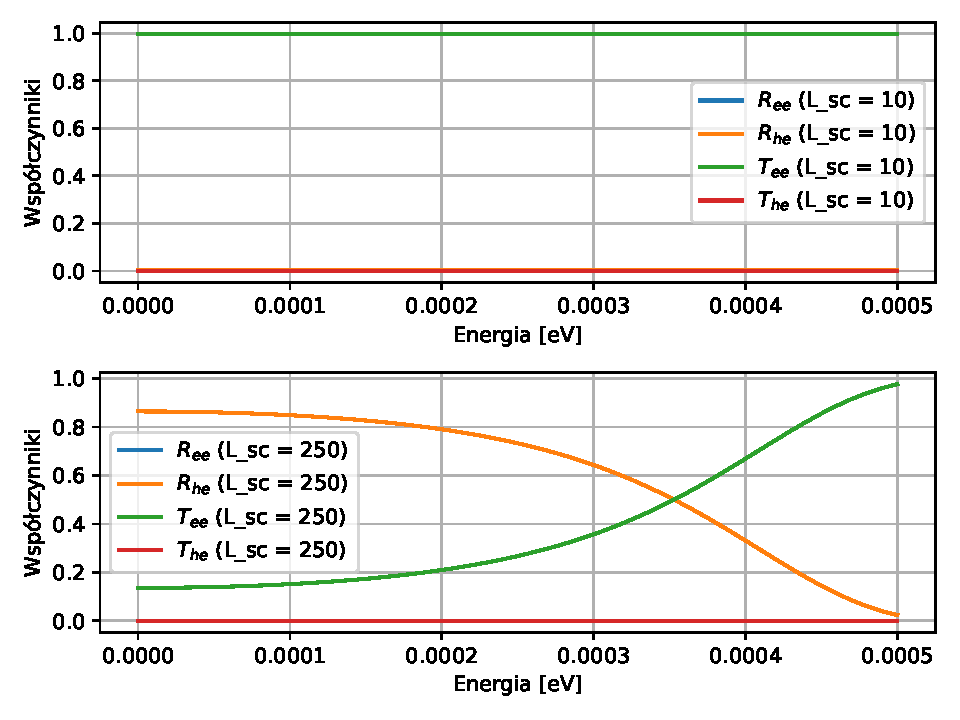
\includegraphics[width=0.65\linewidth]{ex2/ex_fmscfm1_transmission.pdf}
    \caption{ Współczynniki transmisji w funkcji energii padającego elektronu dla złącza NM/SC/NM. Wyniki
dla złącza, w którym długość obszaru SC (góra) LSC = 10 nm oraz (dół) LSC = 250 nm.}
    \label{fig:ex2-transmission}
\end{figure}
Badaliśmy tutaj wpływ szerokości obszaru SC: $L_{\text{sc}}=10, 250$~nm.
Na górnym rysunku ($L_{\text{sc}}=10$~nm) nie obserwujemy zmian żadnych ze współczynników w funkcji rozpatrywanych energii.
Z kolei na dolnym rysunku ($L_{\text{sc}}=250$~nm) wraz ze wzrostem energii, maleje wartość odbicia Andreeva i rośnie współczynnik transmisji elektron--elektron.\\
\\
Zbadaliśmy następnie wpływ szerokości $L_{\text{sc}}$ na powyższe współczynniki przy stałej energii poniżej przerwy nadprzewodzącej, np.~$E = 0.1e-03$.
Dane zależności zostały zapisane na rysunku~\ref{fig:ex2-wspolczynniki-lsc}.
\begin{figure}[htp!]
    \centering
    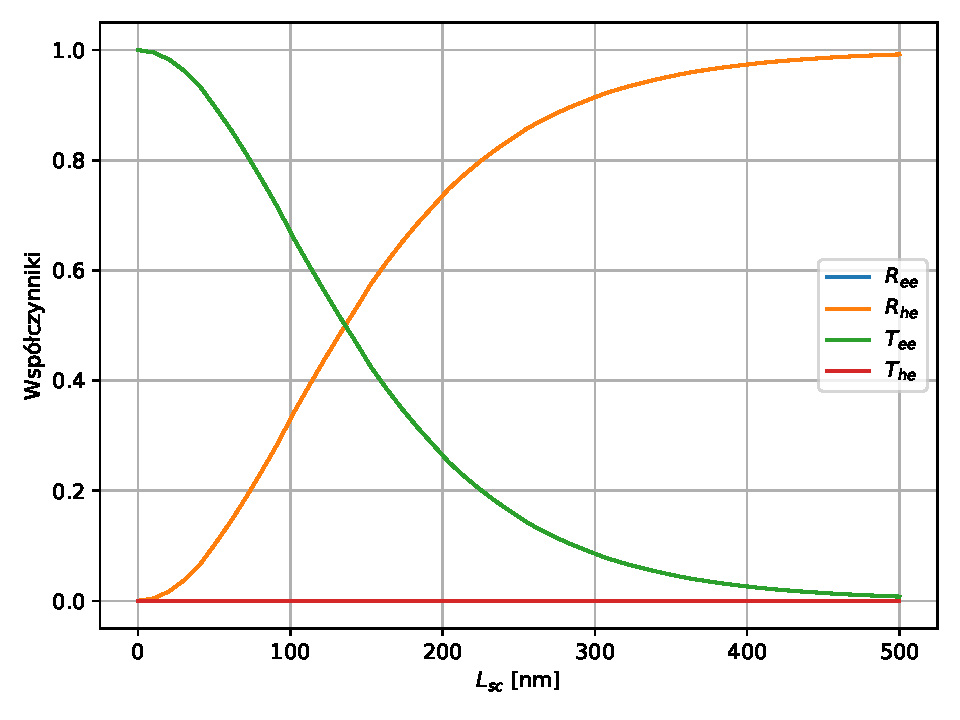
\includegraphics[width=0.65\linewidth]{ex2/ex_fmscfm2_transmission_vs_L_sc.pdf}
    \caption{Współczynniki transmisji w funkcji długości obszaru nadprzewodzącego LSC dla złącza NM/SC/NM.
Wyniki dla energii padającego elektronu E = 0.1 meV}
    \label{fig:ex2-wspolczynniki-lsc}
\end{figure}
Obserwujemy, że wraz ze wzrostem długości $L_{\text{SC}}$ rośnie współczynnik odbicia Andreeva $R_{he}$, natomiast transmisja elektron-elektron $T_{ee}$ maleje.\\
\\
Na koniec przeanalizowano przypadek asymetrycznego kontaktu: $P_l = 0.995$, $P_r = 0$, przy tej samej energii $E = 0.1$ meV. 
Wyniki przedstawiono na rysunku~\ref{fig:ex2-transmission-pl}.
\begin{figure}[htp!]
    \centering
    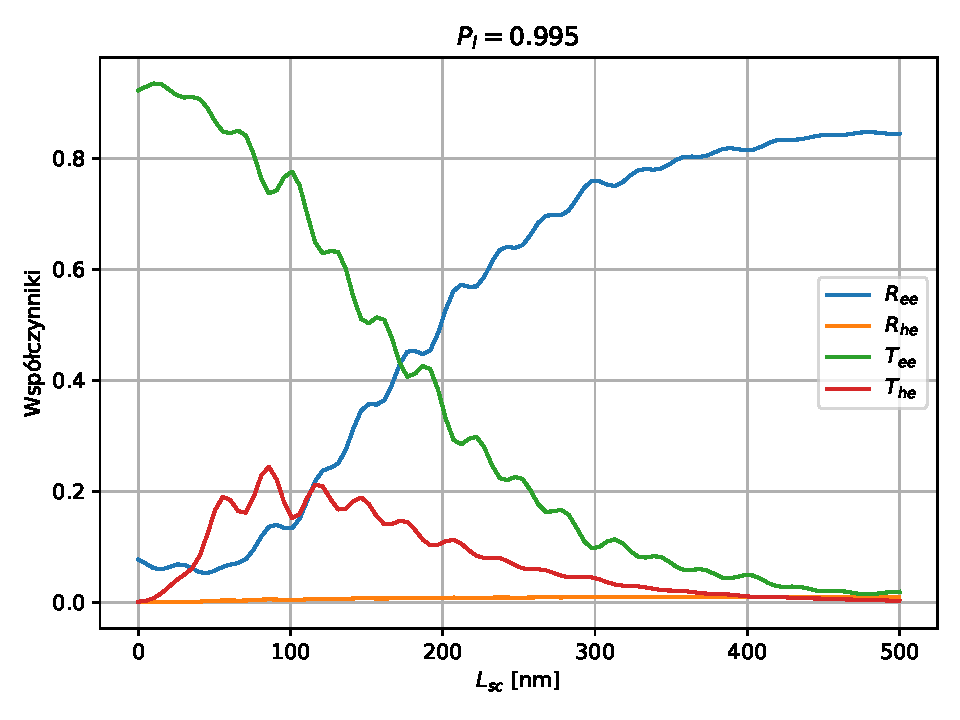
\includegraphics[width=0.65\linewidth]{ex2/ex_fmscfm3_transmission_vs_L_sc.pdf}
    \caption{Współczynniki transmisji w funkcji długości obszaru nadprzewodzącego LSC dla złącza NM/SC/NM.
Wyniki dla energii padającego elektronu $E = 0.1~\text{ meV}, P_r = 0. \text{ oraz }  P_l = 0.995$}
    \label{fig:ex2-transmission-pl}
\end{figure}
W tym przypadku współczynnik transmisji elektron-elektron $T_{ee}$ ponownie maleje z długością SC, natomiast pojawia się również niezerowy składnik transmisji elektron-dziura $T_{he}$ dla krótszych długości $L_{\text{SC}}$. 
Może to świadczyć o występowaniu skośnych odbić Andreeva.
%%%%%%%%%%%%%%%%%%%%%%%%%%%%%%%%%%%%%%%%%%%%%%
\section{Podsumowanie}
%%%%%%%%%%%%%%%%%%%%%%%%%%%%%%%%%%%%%%%%%%%%%%
W ramach ćwiczenia badano nanostruktury typu NM/SC oraz NM/SC/NM, koncentrując się na zjawisku odbicia Andreeva oraz wpływie parametrów takich jak długość obszaru nadprzewodzącego i spinowa polaryzacja kontaktów na współczynniki transmisji i odbicia.
\end{document}
